\chapter{Tandem mass spectrometry for disulphide bond analysis}

In this chapter we describe differences in \gls*{ms} instrumentation, especially in the context of \gls*{db} mapping. The specific instrumentation choices that were made during preparation of the analysed data are relevant for the construction of the \gls*{db} identification algorithm.

In the introduction we have established that \glspl*{db} are important to protein function, structure, and to enzyme regulation. We have also shown that information about their positions can be used to optimize folding methods that are based on molecular dynamic simulations. We hope that these are enough to persuade the reader that studying the \gls*{db} positions in a protein is a worthwhile task, although a complicated one.

The most popular method of \gls*{db} mapping is \gls*{msms}. \gls*{msms} is a general analysis technique that is often used in proteomics for its accuracy, sensitivity, and speed~\cite{gorman2002protein}.

In \gls*{msms} analysis (or more accurately its bottom-up variant), the protein is fragmented to smaller charged peptides whose mass to charge ratio (\(m/z\)) is measured with atomic precision. Multiple sets of \emph{fragmentation spectra} are obtained, each coming from a longer peptide with a specific \(m/z\) value that is called the \emph{precursor}. While in proteomics the task is usually to identify the original protein from the fragments, during \gls*{db} mapping it is known which protein the fragments come from, and instead the task is to determine the positions of its \glspl*{db}.

The experiment can be designed in a way that keeps the \glspl*{db} intact, resulting in the occurrence of cross-linked peptides with specific fragmentation signatures. There are multiple analytical methods that try to discover these fragmentation spectra and use them to determine the positions of the \glspl*{db} in the protein. Other methods choose to dissociate the \glspl*{db} during the fragmentation, a process that leads to another kind of specific fragmentation signatures.

The first few sections of this chapter roughly reflect the first few steps in a \gls*{ms} experiment.

\begin{enumerate}
  \item The first topic we discuss is sample preparation, an important prerequisite in bottom-up mass spectrometric analysis (\Cref{sec:trypsin}).
  \item In \Cref{sec:lc}, a short overview of sample separation methods is provided.
  \item With the sample being digested and separated, we move on to explain the principles behind \gls*{ms} itself, putting the focus on methods and techniques that are relevant to \gls*{db} analysis (\Cref{sec:msms}). Where possible, we compare multiple methods and state their trade-offs in the context of our work.
  \item Finally, we list some current approaches to \gls*{db} mapping, noting their respective strengths and weaknesses (\Cref{sec:analysis}). At the very end of this chapter, we reformulate the task in more formal terms and roughly approximate its computational complexity.
\end{enumerate}

\section{Protein digestion and sample preparation}\label{sec:trypsin}

In order for the protein to be successfully analysed, it first needs to be digested into smaller peptides; trypsin, and, to a lesser extent, pepsin, are popular choices in proteomics.

Trypsin is a serine protease that cleaves amino acid chains at the carboxylic side of lysine and arginine, provided they are not followed by proline~\cite{olsen2004trypsin}. Lysine and arginine are both relatively abundant in most proteins which makes the tryptic digestion peptides --- or as we will call them, \emph{tryptides} --- reasonably sized for a \gls*{ms} analysis~\cite{matthiesen2007mass}. Additionally, trypsin has very high specificity, and thus the digestion peptides are quite predictable. However, the sample protein is not cleaved at every potential cleavage site; so-called \emph{missed cleavages} do occur during most proteolytic digestions. The frequency of missed cleavages depends on neighbouring residues of the cleavage site~\cite{gershon2014cleaved}, the used protease, and the experimental setup.

An interesting particularity of trypsin and some other proteases is relevant to our work: they require a neutral-to-basic environment in order to become proteolytically active. In this type of environment the issue of \gls*{db} scrambling arises~\cite{wu1997novel}; some \glspl*{db} become dissociated, then the cysteines re-connect, but in different patterns than before. These scrambled bonds are difficult to discern from the naturally occurring ones in the mass spectra. The issue can be mitigated by using a different protease for the digestion, such as pepsin, or thermolysin~\cite{sung2016evaluation}.

In addition to digestion, in a general proteomic experiment the protein usually undergoes reduction that completely dissociates the \glspl*{db}, and cysteine alkylation that prevents the cysteines from reassociating. However, in an experiment that aims to characterize cysteine linkages, only the alkylation is performed, and the present \glspl*{db} are kept intact.

\section{Liquid chromatography sample separation}\label{sec:lc}

In a general proteomic experiment, the signal from more abundant sample peptides may interfere with the other, less frequent ones. To sidestep this problem, it has become routine to perform separation before the main \gls*{ms} experiment, either on the protein level or the peptide level. After separation, fewer analytes are present in a mass spectrometer at a given point in time, reducing the chance of a signal becoming lost. Protein-level separation is common among experiments with the goal of identifying which proteins are present in the sample; in the case of \gls*{db} characterization, there is only one protein present, so peptide-level separation is the method of choice.

A popular peptide-level separation method is \gls*{lc}. In a model proteomic \gls*{ms}-\gls*{lc} experiment, the proteins are digested without prior separation, and the resulting peptides are separated on reverse-phase \gls*{lc} column that is directly connected to a tandem mass spectrometer~\cite{washburn2001large}. This process is applicable to \gls*{db} analysis as well.

Reverse-phase \gls*{lc} has two main constituents: a mobile liquid phase that contains the peptides, and a stationary solid phase which is usually a nonpolar column with \(\ce{C18}\) alkyl chains~\cite{chang1976high}. The mobile phase passes along the stationary phase, the elution time of each individual peptide depending on its hydrophobic interactions with the alkyl chains. The peptides are eluted with a polar mixture of water and organic solvent, such as acetonitrile~\cite{frohlich2006proteome}, the shortest and least hydrophilic peptides eluting the earliest.

The \gls*{lc} column is often directly connected to the mass spectrometer, which performs the bulk of the analysis.


\section{Tandem mass spectrometry}\label{sec:msms}

\Gls*{ms} is an analytical technique that has originally been used for studying small thermostable molecules. Nevertheless, with the advancements in soft ionization allowing proteins and other biomolecules to be analysed as well~\cite{fenn1989electrospray}, \gls*{ms} has become an indispensable tool in proteomics research~\cite{collins2003human}.

\Gls*{ms} experiments can be either single-stage (\gls*{ms}) or tandem, the latter being denominated \gls*{msms}, sometimes \gls*{ms}\textsuperscript{2}, and in the cases of more than two subsequent analyses, \gls*{ms}\textsuperscript{\(n\)}. During single-stage experiments, the mass distribution of a polypeptide sample is determined. The more frequent of the two, \gls*{msms} is used to learn about certain structural features of a protein, including sequence and \glspl*{ptm}~\cite{domon2006mass}.

\begin{figure}
  \centering
  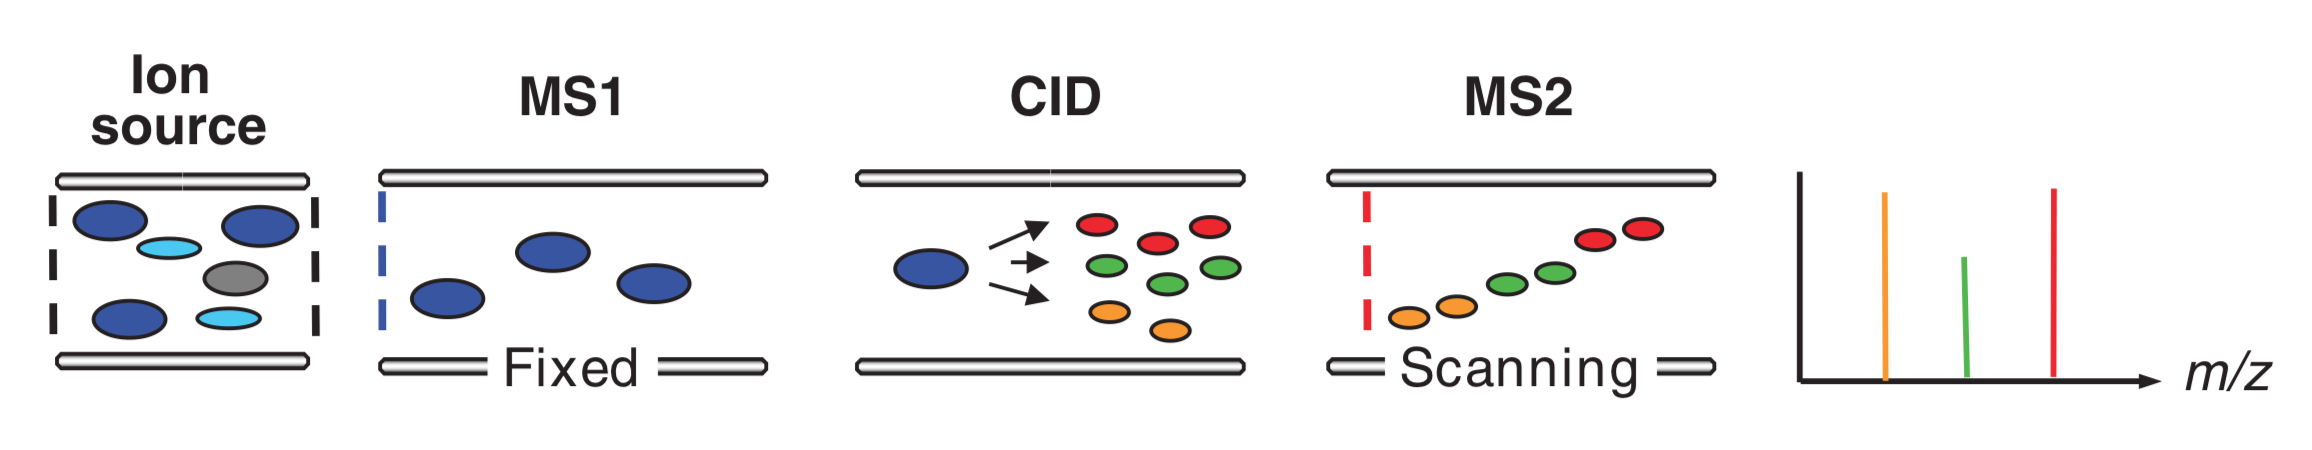
\includegraphics[width=.9\linewidth]{img/msms-workflow.png}
  \caption{A diagram of an ordinary \gls*{msms} workflow. While the specific instrumentation details differ from spectrometer to spectrometer, the general structure of ionize \textrightarrow{} analyse \textrightarrow{} fragment \textrightarrow{} analyse is common to all \gls*{msms} experiments. Image by~\citet{domon2006mass}.}\label{fig:mass-spectrometry-workflow}
\end{figure}

Both the single-stage and \gls*{msms} experiments begin similarly: the sample peptides are ionized (see \Cref{sec:ionization}), and the ions travel through an electromagnetic field in an analyser whilst their mass-to-charge (\(m/z\)) is being calculated (\Cref{sec:msms-analysis})~\cite{gross2006mass}. In single-stage \gls*{ms}, the experiment ends there, while in \gls*{msms}, some of these \emph{precursors} are selected to undergo fragmentation in the collision cell (\Cref{sec:fragmentation}); the typical \gls*{msms} workflow is shown in \Cref{fig:mass-spectrometry-workflow}. The resulting fragments are analysed and their \(m/z\) values noted; the output of the \gls*{msms} experiment is made of precursors with their masses and their fragmentation spectra; an example of a precursor fragmentation spectrum can be seen on figure \Cref{fig:frag-spectrum}.

\begin{figure}
  \centering
  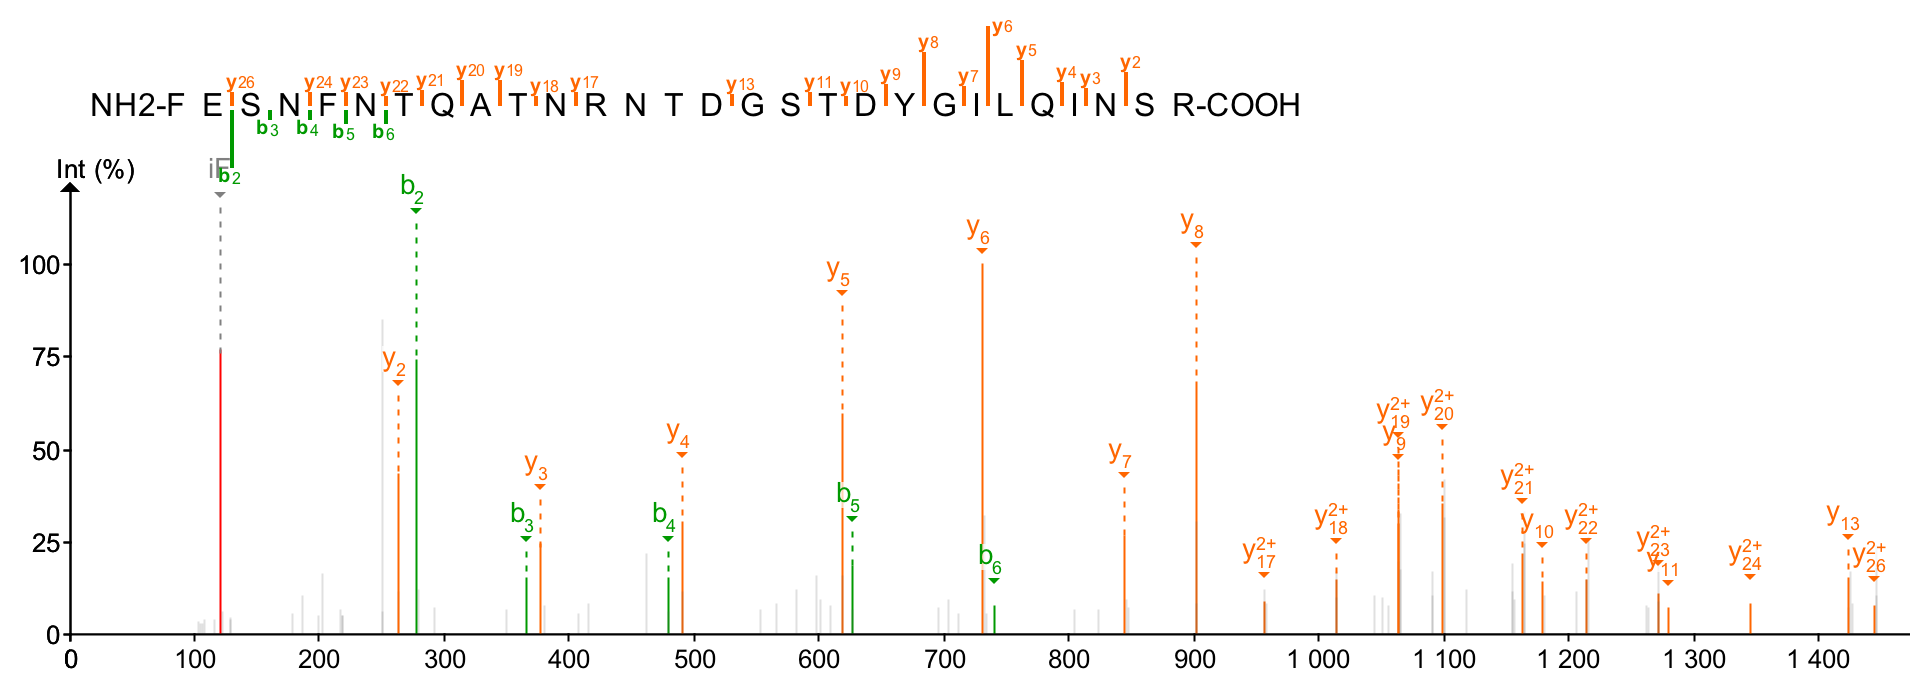
\includegraphics[width=1\linewidth]{img/fragmentation-spectrum.png}
  \caption{An annotated fragmentation spectrum of the precursor \emph{FESNFNTQATNRNTDGSTDYGILQINSR}. A \emph{peak} signifies that a peptide with a specific \(m/z\) value has been seen, and also provides information about the intensity of its signal.}\label{fig:frag-spectrum}
\end{figure}

When the analysed protein is cross-linked by \glspl*{db}, some precursors will be cross-linked, too. The aim of the \gls*{db} \gls*{msms} analysis is to identify the cross-linked precursors and deduce the positions of \glspl*{db} in the protein. Specific instrumentation choices influence the behaviour of cross-linked peptides during the analysis, and result in fragmentation spectra with vastly different characteristics. Sometimes one approach is preferable; for example in the case of picking an analyser, Orbitrap is usually preferred thanks to its accuracy and sensitivity. Other times the choice is more ambiguous, such as the choice between \gls*{cid} and \gls*{etd} fragmentation. We discuss the possible instrumentation choices in the context of \gls*{db} mapping in the following sections; the overview is partly based on the works of \citet{matthiesen2007mass} and \citet{gross2006mass}.

\subsection{Sample ionization}\label{sec:ionization}

Only charged compounds in gas phase are detectable by a mass spectrometer analyser. If the samples are not in this form, they need to be ionized.

One of the oldest ionization methods is electron ionization (EI)~\cite{field2013electron}. However, EI is unsuitable for large thermally unstable organic molecules, such as peptides; for proteomics work, the two most popular options are \gls*{maldi} and \gls*{esi}~\cite{caprioli1997molecular, fenn1990electrospray}.\@ Unlike \gls*{esi}, the \gls*{maldi} ionization process has to be done in a vacuum, making it impossible to directly connect a \gls*{lc} column to the spectrometer. Thus, for the purpose of \gls*{db} mapping, \gls*{esi} is usually the ionization method of choice.

During \gls*{esi}, a very fine capillary with a solution that contains the sample peptides and charged ions is placed into a strong electrostatic field. Due to the influence of the field, the solution forcibly squirts out of the capillary, creating a mist of miniscule charged droplets. The solution slowly evaporates from the droplets, until eventually the repulsive electric forces inside the droplet overcome its surface tension and the droplet splits into yet smaller droplets~\cite{rayleigh1882xx}. This evaporating and splitting process repeats itself, until we are left with isolated sample ions in the gas phase~\cite{dole1968molecular,dole1968gas,fenn1989electrospray, fenn1990electrospray}.

For our work, three properties of \gls*{esi} are important.

\begin{itemize}
  \item \gls*{esi} works under atmospheric pressure, enabling the \gls*{lc} colon to be connected directly to the mass spectrometer, creating an ``online'' or ``hyphenated'' \gls*{lc}-\gls*{ms} system~\cite{opiteck1997comprehensive}. This property simplifies the \gls*{msms} experiment and provides higher throughput.
  \item The ionization cases very little to no fragmentation to the sample~\cite{griffiths2001electrospray} --- in other words, \gls*{esi} a ``soft'' ionization technique. This property is useful because it simplifies the subsequent analysis, and does not add noise to the measured information.
  \item  Ions generated by \gls*{esi} are often multiply charged~\cite{felitsyn2002origin}, bringing their \(m/z\) value down and enabling us to analyse peptides with a higher mass in an ordinary mass spectrometer setting.
\end{itemize}

\subsection{Mass analysers}\label{sec:msms-analysis}

A mass analyser, sometimes equipped with a separate detector, measures the mass to charge ratio (\(m/z\)) and intensity of a sample compound. The many existing mass analysers differ in the principle of function, and their performance characteristics.

\begin{description}
  \item[Time-of-flight analyser] In TOF analysers~\cite{stephens1946pulsed}, sample ions are accelerated with an electric field to make them travel along a path with known length. The ions with lower \(m/z\) values will arrive measurably sooner than the ones with higher \(m/z\) values, as long as all of them are dispersed at a similar-enough points in time. Due to this requirement, TOF analysers are best suited for pulsed ionization techniques such as \gls*{maldi}\@. TOF analysers have an excellent sensitivity and, at least in theory, their \(m/z\) range is unlimited~\cite{fuerstenau1995molecular}.
  \item[Linear quadrupole analyser] As the name suggest, a linear quadrupole consist of four linear rods which are placed parallel to each other and arranged in a square shape, see \Cref*{fig:quadrupole}. A pair of rods sitting in diagonally opposite corners has the same polarity, however, the pairs periodically switch the polarity. An ion travelling along the rods is periodically repelled and attracted to each of the rods, its precise trajectory depending on its \(m/z\) value~\cite{paul1990electromagnetic}. In this way, ions with specific \(m/z\) values can pass through the quadrupole into a detector~\cite{paul1953neues}, while others follow an unstable trajectory and crash into one of the poles or the wall of the quadrupole.

    Quadrupoles can also trap specific ions inside instead of making them simply pass through; such quadrupole is usually called a linear ion trap~\cite{mao2003h}. Furthermore, quadrupoles can serve as fragmentation collision cells. Due to their flexibility, a tripple-quadrupole mass spectrometer was a popular choice for \gls*{msms} experiments~\cite{yost1978selected}.
  \item[FT-ICR analyser] In Fourier transform ion cyclotron resonance analysers (FT-ICR) the analytes circulate in a magnetic field, and Fourier transform is used to decode the induced signals. The \(m/z\) values are calculated from the frequencies and amplitudes~\cite{comisarow1974fourier}. Many ions with wildly different \(m/z\) values can be measured in parallel, making the analysis faster. Further improvements also increased the mass accuracy and resolution beyond what is attainable by quadrupole analysers~\cite{amster1996fourier, easterling1999routine}.
  \item[Orbitrap analyser] The Orbitrap is the most important analyser type in the context of our work~\cite{hu2005orbitrap}. It achieves similar accuracy, resolving power, and dynamic range to FT-ICR, but does not require an expensive-to-run supra-conducting magnet to do so. In Orbitrap the ions simultaneously cycle around the centre and oscillate along the z-axis, as is illustrated on \Cref*{fig:orbitrap}. This oscillation induces a periodically changing electrical current in the detector that is converted to an \(m/z\) spectrum of the analyte with the help of Fourier transform.

    The Orbitrap often achieves sub-ppm error rates, which makes it ideal for our use case. Our goal is to identify complicated ions, and for that we need the measurements of their mass to be as reliable as possible. Furthermore, it is possible to connect Orbitrap to a \gls*{esi} ion source, and by extension to a \gls*{lc} colon.
\end{description}

\begin{figure}
  \centering
  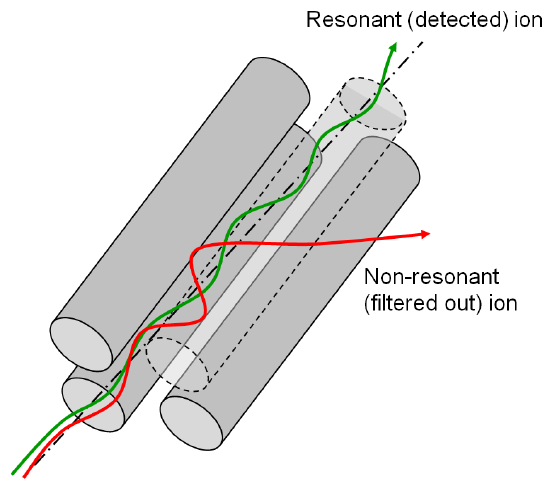
\includegraphics[width=.4\linewidth]{img/quadrupole.png}
  \caption{A quadrupole with two highlighted classes of ion trajectories. The ion with green trajectory passes through the quadrupole and is ultimately detected, while the one with the red trajectory is filtered out. How will the trajectory look like for a specific ion depends on its \(m/z\) value. Image taken from~\citet{2021Mass}.}\label{fig:quadrupole}
\end{figure}

\begin{figure}
  \centering
  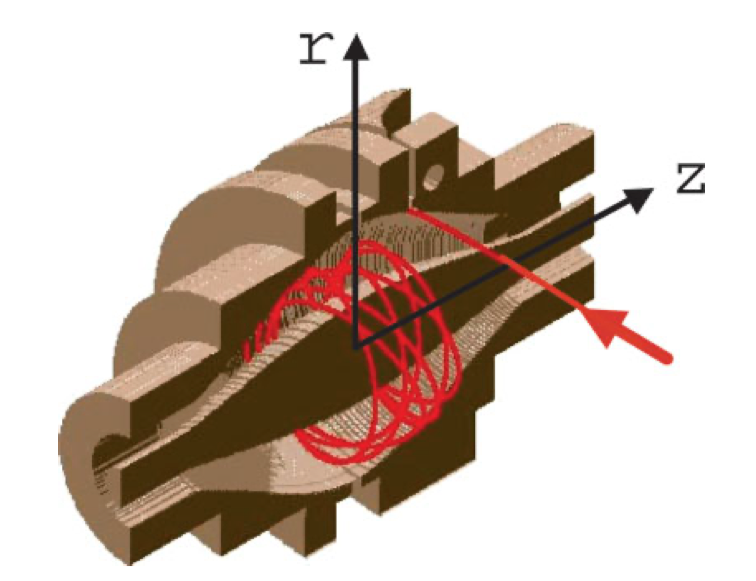
\includegraphics[width=.5\linewidth]{img/orbitrap.png}
  \caption{An Orbitrap mass analyser with a typical ion trajectory highlighted. The ion circulates around the centre while simultaneously oscillating along the z-axis. The oscillation is detected and used to compute the \(m/z\) value of the ion. Image by~\citet{hu2005orbitrap}.}\label{fig:orbitrap}
\end{figure}

\subsection{Precursor fragmentation}\label{sec:fragmentation}

In \gls*{msms} experiments, once the mass spectrum of the initial sample is analysed and the \gls*{ms}\textsuperscript{1} data are acquired, \emph{precursors} are selected according to their mass, and fragmented. The fragments undergo yet another mass analysis, producing so called \gls*{ms}\textsuperscript{2} data. In the section we present a short overview of the currently used fragmentation methods.

When the goal of the experiment is to observe \glspl*{ptm} and to preserve the volatile bond connecting the \gls*{ptm} to the peptide, \gls*{ecd}~\cite{zubarev2000electron} or \gls*{etd}~\cite{syka2004peptide} are preferred. Both methods use electron transfer to induce amine backbone bond cleavage that results in the creation of \(c\) and \(z\) ions, as illustrated in \Cref{fig:fragment-types}.

During \gls*{etd}, the \glspl*{db} are dissociated, and the cross-linked precursor is split into its constituent peptides~\cite{liu2014facilitating}. These peptides appear as high-intensity peaks in the fragmentation spectra. The peaks which can be used to determine the peptide makeup of the original precursor, which causes \gls*{etd} to be a popular fragmentation technique in \gls*{db} mapping methods. However, if the precursor contains multiple cysteines, it may be hard to deduce which of them were paired together, especially if there were multiple \glspl*{db} present. In this work we focus on methods that do not have this disadvantage.

First of these methods is \gls*{cid}. \gls*{cid} accelerates the precursor ions, and makes them collide with neutral gas molecules, ultimately leading to their fragmentation. The dissociation process usually takes place at the more labile bonds, such as the ones connecting \glspl*{ptm}~\cite{quan2013cid}, or peptide bonds in the precursor backbone.\footnote{The fact that many \gls*{ptm} bonds are preferentially dissociated during \gls*{cid} is usually seen as unfortunate. However, in the case of \gls*{db} mapping it simplifies the analysis, as the \glspl*{ptm} can be safely ignored, which reduces the combinatorial complexity of the problem.} \gls*{cid} produces \(b\) and \(y\) fragment ions (see \Cref{fig:fragment-types}); additionally, as a side effect of the dissociation, a small neutral molecule sometimes breaks off of the fragment, lowering its total mass value without affecting its charge. This dissociated molecule is called a \emph{neutral loss}. In \gls*{cid}, the most common neutral losses are water and ammonia.

A specific variant of \gls*{cid} called the beam-type \gls*{cid} produces \emph{internal ions}, fragments that are generated by two (or more) bond cleavages during the fragmentation. Many of the internal ions begin with a proline~\cite{michalski2012systematic}, suggesting that the double cleavage event prefers some amino acids to others. As shown by \citet{michalski2012systematic}, ion-trap \gls*{cid}, the other \gls*{cid} variant, does not produce internal ions. Furthermore, ion-trap \gls*{cid} has limits regarding the containment of molecules below a certain mass threshold, leading to a mass cut-off~\cite{louris1987instrumentation}.

\begin{figure}
  \centering
  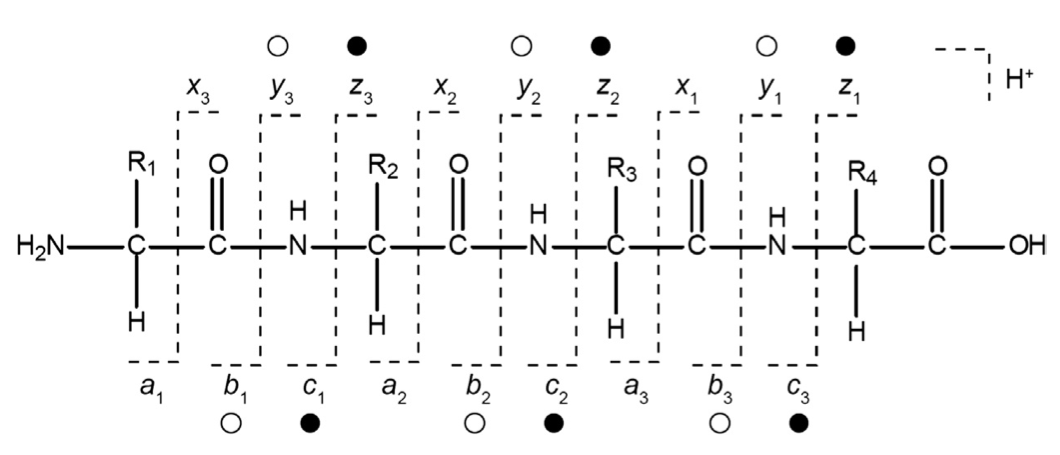
\includegraphics[width=.75\linewidth]{img/fragment-types.png}
  \caption{A singly positively charged peptide with annotated fragmentation types. The \gls*{cid} b/y ion fragments are marked with open circles, while the typical \gls*{ecd} and \gls*{etd} c/z ion fragments are marked with filled circles. Image by~\citet{hart2014review}.}\label{fig:fragment-types}
\end{figure}

A similar fragmentation signature to \gls*{cid} can also be obtained by infrared multiphoton dissociation (IRMPD)~\cite{oomens2006gas}. Because IRMPD, and the related UV-MPD, do not require collision gasses to be present for the fragmentation, they are well suited for analysers operating under high vacuum, such as FT-ICR\@.

In 2007 a new fragmentation method based on beam-type \gls*{cid} has been devised, called the \gls*{hcd}\@. The fragmentation spectra obtained from \gls*{cid} and \gls*{hcd} are very similar~\cite{michalski2012systematic}, nonetheless there is a key difference between the two methods: \gls*{hcd} combines the richer sequence information~\cite{xia2006ion} and lower mass cut-off of beam-type \gls*{cid} with the superior resolution capacity and accuracy of the Orbitrap analyser. That is one of the reasons the data we use in this thesis come from \gls*{hcd}\@. In the next section we describe the common \gls*{hcd} fragmentation pathways, because they are crucial to the function of our \gls*{db} mapping program.

\subsubsection{Fragmentation pathways in \gls*{hcd}}

Fragments from \gls*{esi}-ionized precursors can be and indeed are often multiply charged~\cite{katta1991use, michalski2012systematic}. According to the research on \gls*{cid} of cross-linked peptides by \citet{giese2016study}, most of the cross-linked fragments were found to have a positive charge of at least 2, while an overwhelming majority of linear fragments had a positive charge of 1. \gls*{hcd} is in principle similar to \gls*{cid}, and we believe these findings would translate to \gls*{hcd}-generated fragments as well.

The different types of fragments of a very pure sample were nicely summarized by \citet{michalski2012systematic}. Ions of \(b\), \(y\) and \(a\) type comprise most of the spectral intensity (54\%, see \Cref{fig:hcd}). The ions themselves have different distributions, the \(y\) type being the most abundant. Other neutral loss ions, be it a loss of water, ammonia, or an amino-acid-specific small molecule\footnote{If specific amino acid neutral losses are of interest, the review by~\citet{paizs2005fragmentation} lists many of them.}, together with internal ions, can be attributed a quarter of the total fragment intensity. Finally, immonium ions account for 6\% of the intensity. In total 85\% of the spectral intensity is explainable. For a visual overview of the many \gls*{hcd} fragmentation types, please refer to \Cref{fig:fragment-types-hcd}.

\begin{figure}
  \centering
  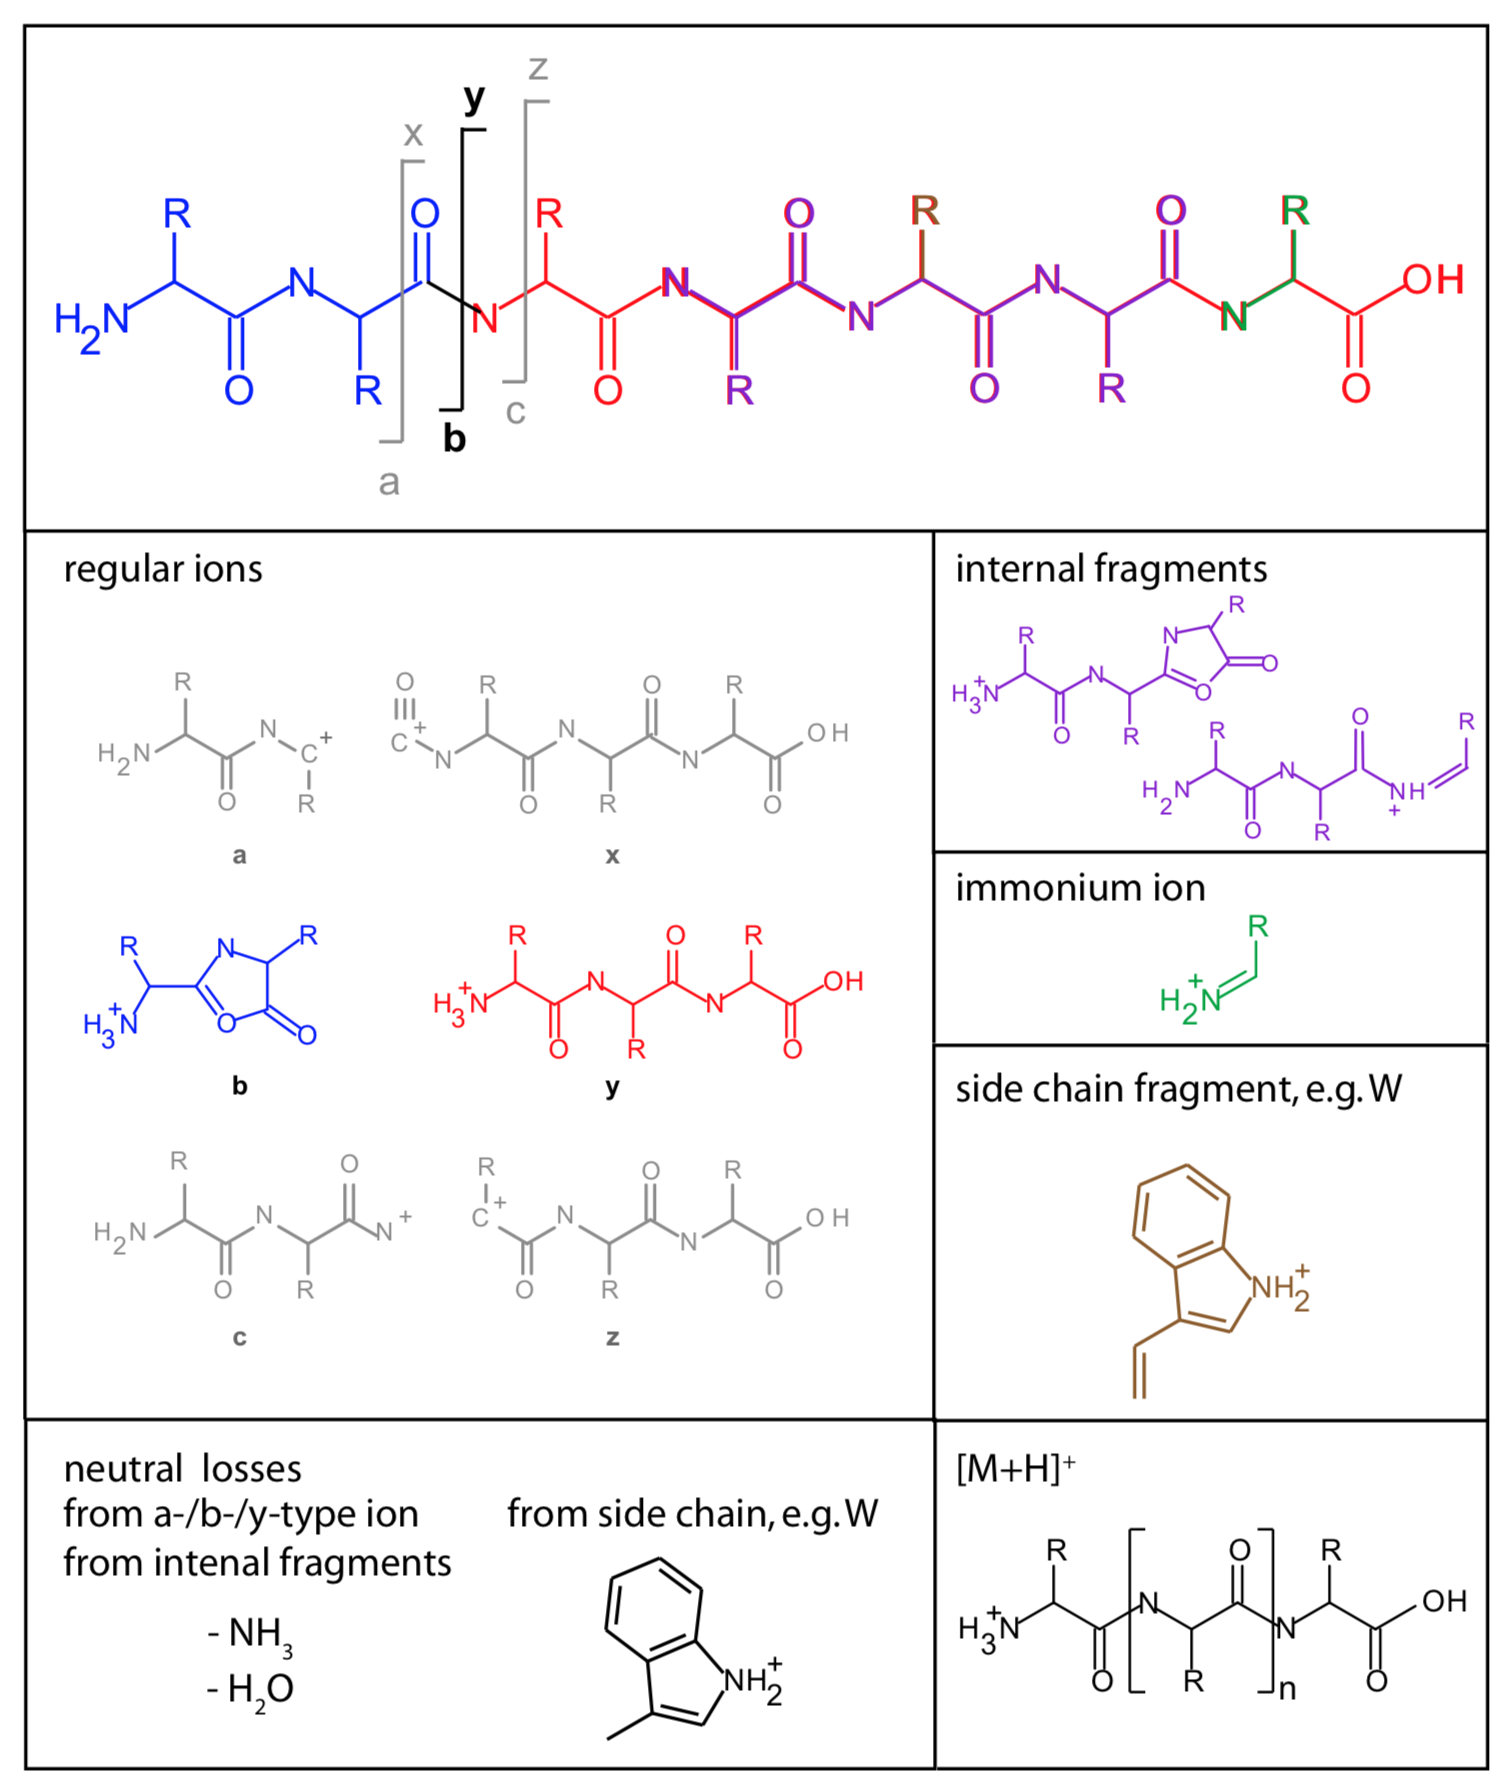
\includegraphics[width=.9\linewidth]{img/fragment-types-hcd.png}
  \caption{The different fragment types that are common in \gls*{hcd} fragmentation. During \gls*{hcd}, \(b, y\), and to a lesser extent \(a\), ions are the most frequent, together with internal ions and immonium ions, and their counterparts with neutral losses. Image by~\citet{michalski2012systematic}.}\label{fig:fragment-types-hcd}
\end{figure}

\begin{figure}
  \centering
  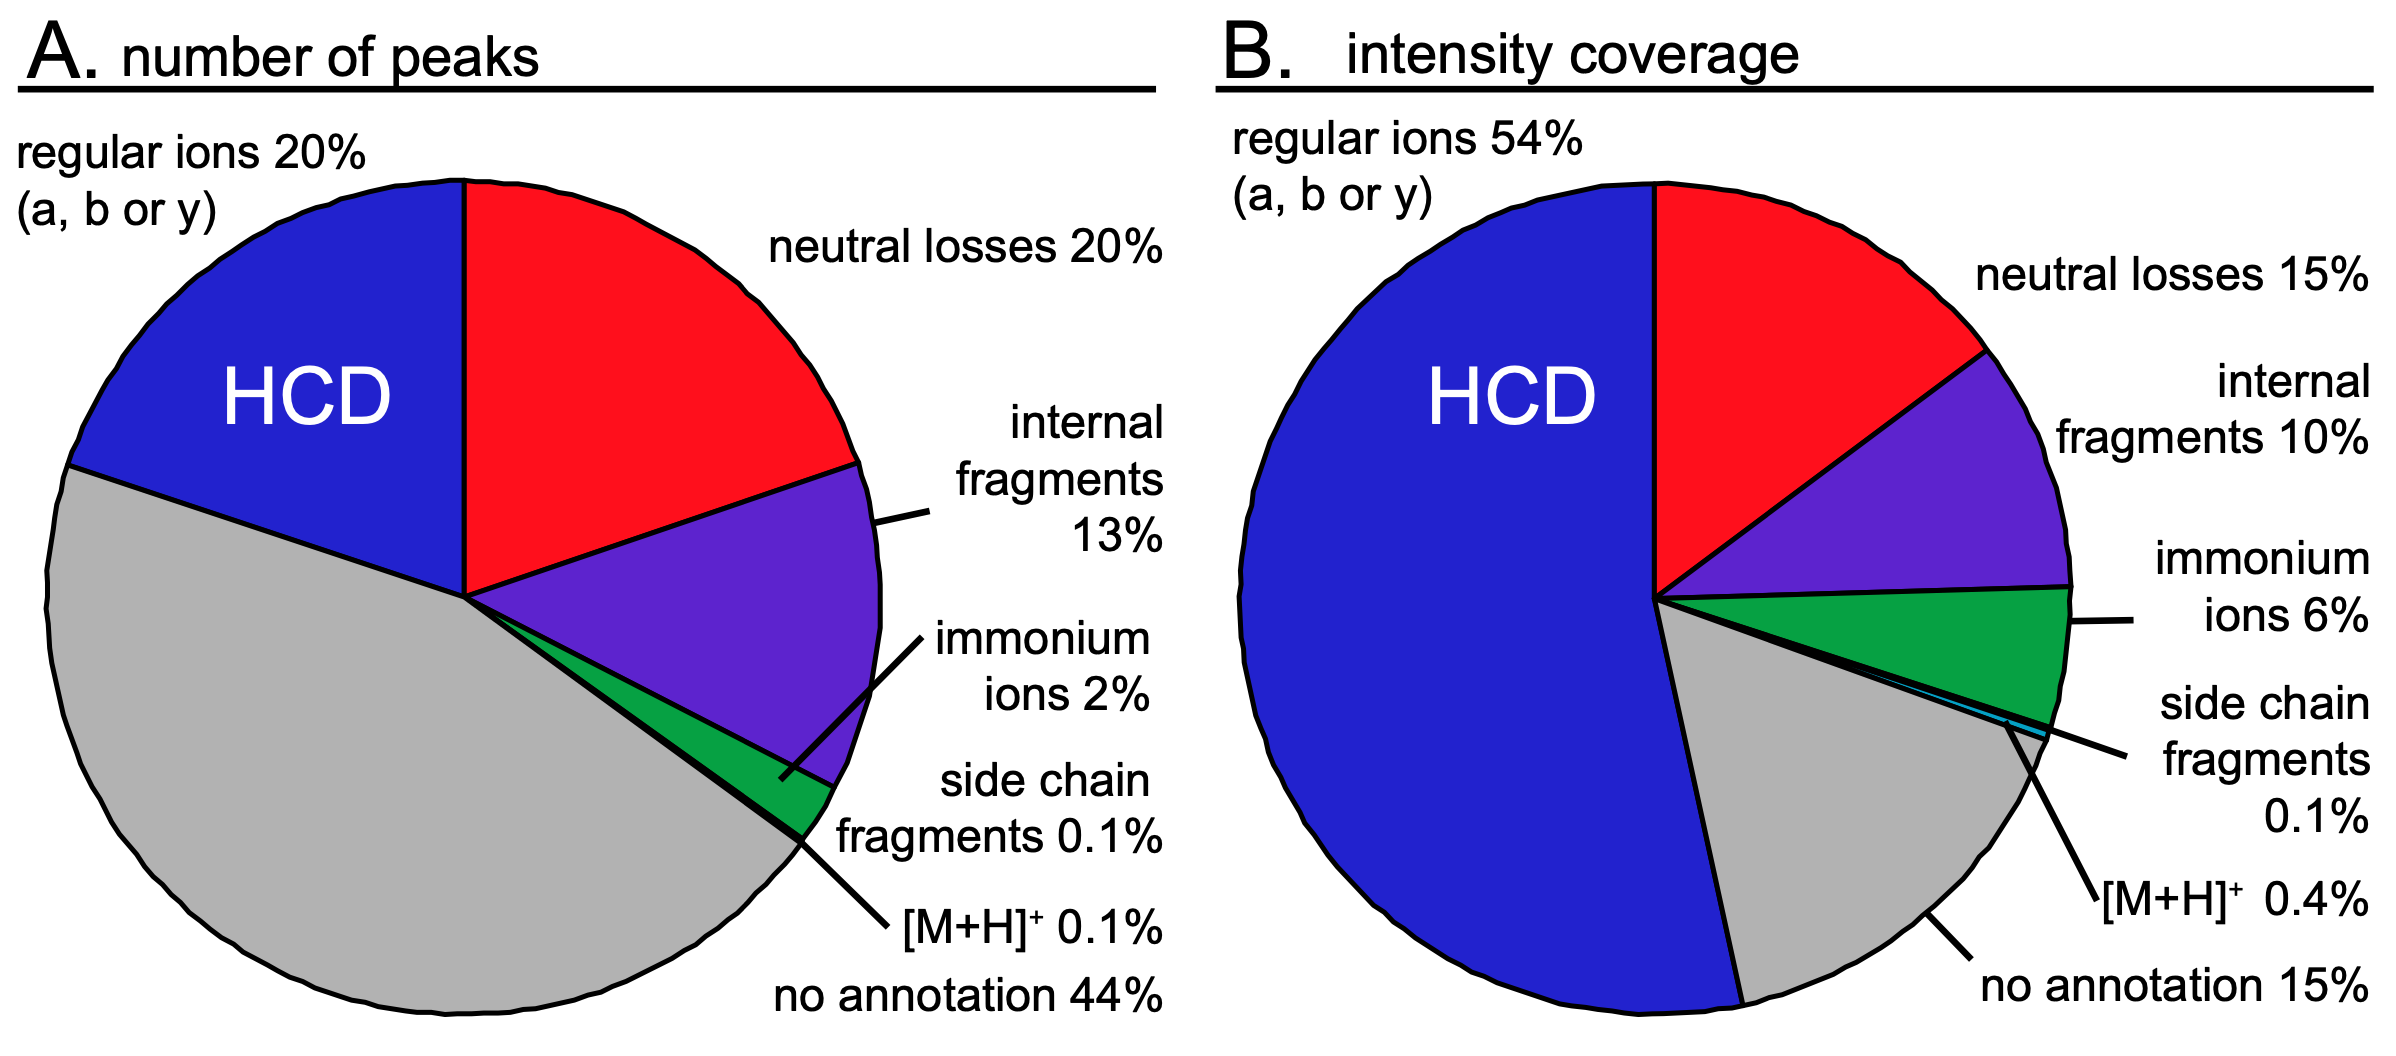
\includegraphics[width=.9\linewidth]{img/hcd.png}
  \caption{(B) In a \gls*{hcd} fragmentation spectrum, \(b, y\), and \(a\) ions are responsible for 54\% of the measured spectral intensity. Another 25\% is generated by fragments with neutral-loss and internal fragments, and another 6\% by immonium ions. Together, those four account for 85\% of the measured intensity. It is true that almost a half of the peaks are still left unexplained (A), however, given all of these fragments have to split the remaining 15\% of intensity, they are probably rather rare and are only of moderate importance. Image by~\citet{michalski2012systematic}.}\label{fig:hcd}
\end{figure}

Although \glspl*{db} are not affected by low-energy \gls*{cid} as much as the other \glspl*{ptm}~\cite{paizs2005fragmentation, lioe2007novel}, in high energy collision fragmentation such as \gls*{hcd}, cleavage of the S-S bond can be observed with a higher probability~\cite{bean1992characterization}. The cleavage of the bond can result in the formation of an asymmetrical distribution of mass on the two cysteines~\cite{zhang2006mapping}, see \Cref{fig:disulphide-bond-cleavage-assymetry} for details. Additionally, the sole presence of a \gls*{db} influences the fragmentation pathways of the whole peptide; \citet{mormann2008fragmentation} reports a low but detectable signal of peptide backbone cleavages in the bonds inside S-S loop of an internal \gls*{db}, while \citet{clark2011collision} reports a higher frequency of internal ions.

\begin{figure}
  \centering
  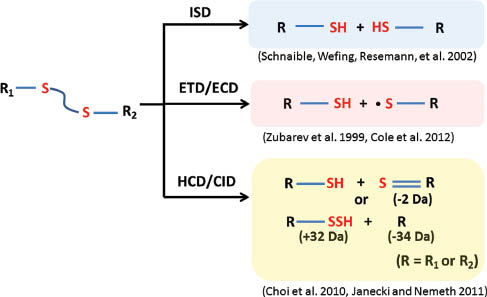
\includegraphics[width=.6\linewidth]{img/disulfide-bond-cleavage-assymetry.jpg}
  \caption{Under different dissociation strategies, \glspl*{db} manifest different cleavage characteristics. Under \gls*{cid}, the cleavage results into two possible asymmetrical mass distributions. Image by~\citet{tsai2013mass}.}\label{fig:disulphide-bond-cleavage-assymetry}
\end{figure}

To recapitulate, in theory a \(b\), \(y\), \(a\), or an internal ion can be seen in a \gls*{hcd} fragmentation spectra with zero or more of the following modifications:

\begin{enumerate}
  \item Dissociated neutral loss.
  \item Covalent modifications on some amino acid residues, such as methionine oxidation. A subset of these are the cysteine alkylations.
  \item A piece of a former \gls*{db} that has been cleaved during the fragmentation.
  \item One or more fragments, possibly modified with some above, connected by a set of \glspl*{db}. For some examples of cross-linked fragments, see \Cref{fig:intra-peptide-bonds}.
\end{enumerate}

\begin{figure}
  \centering
  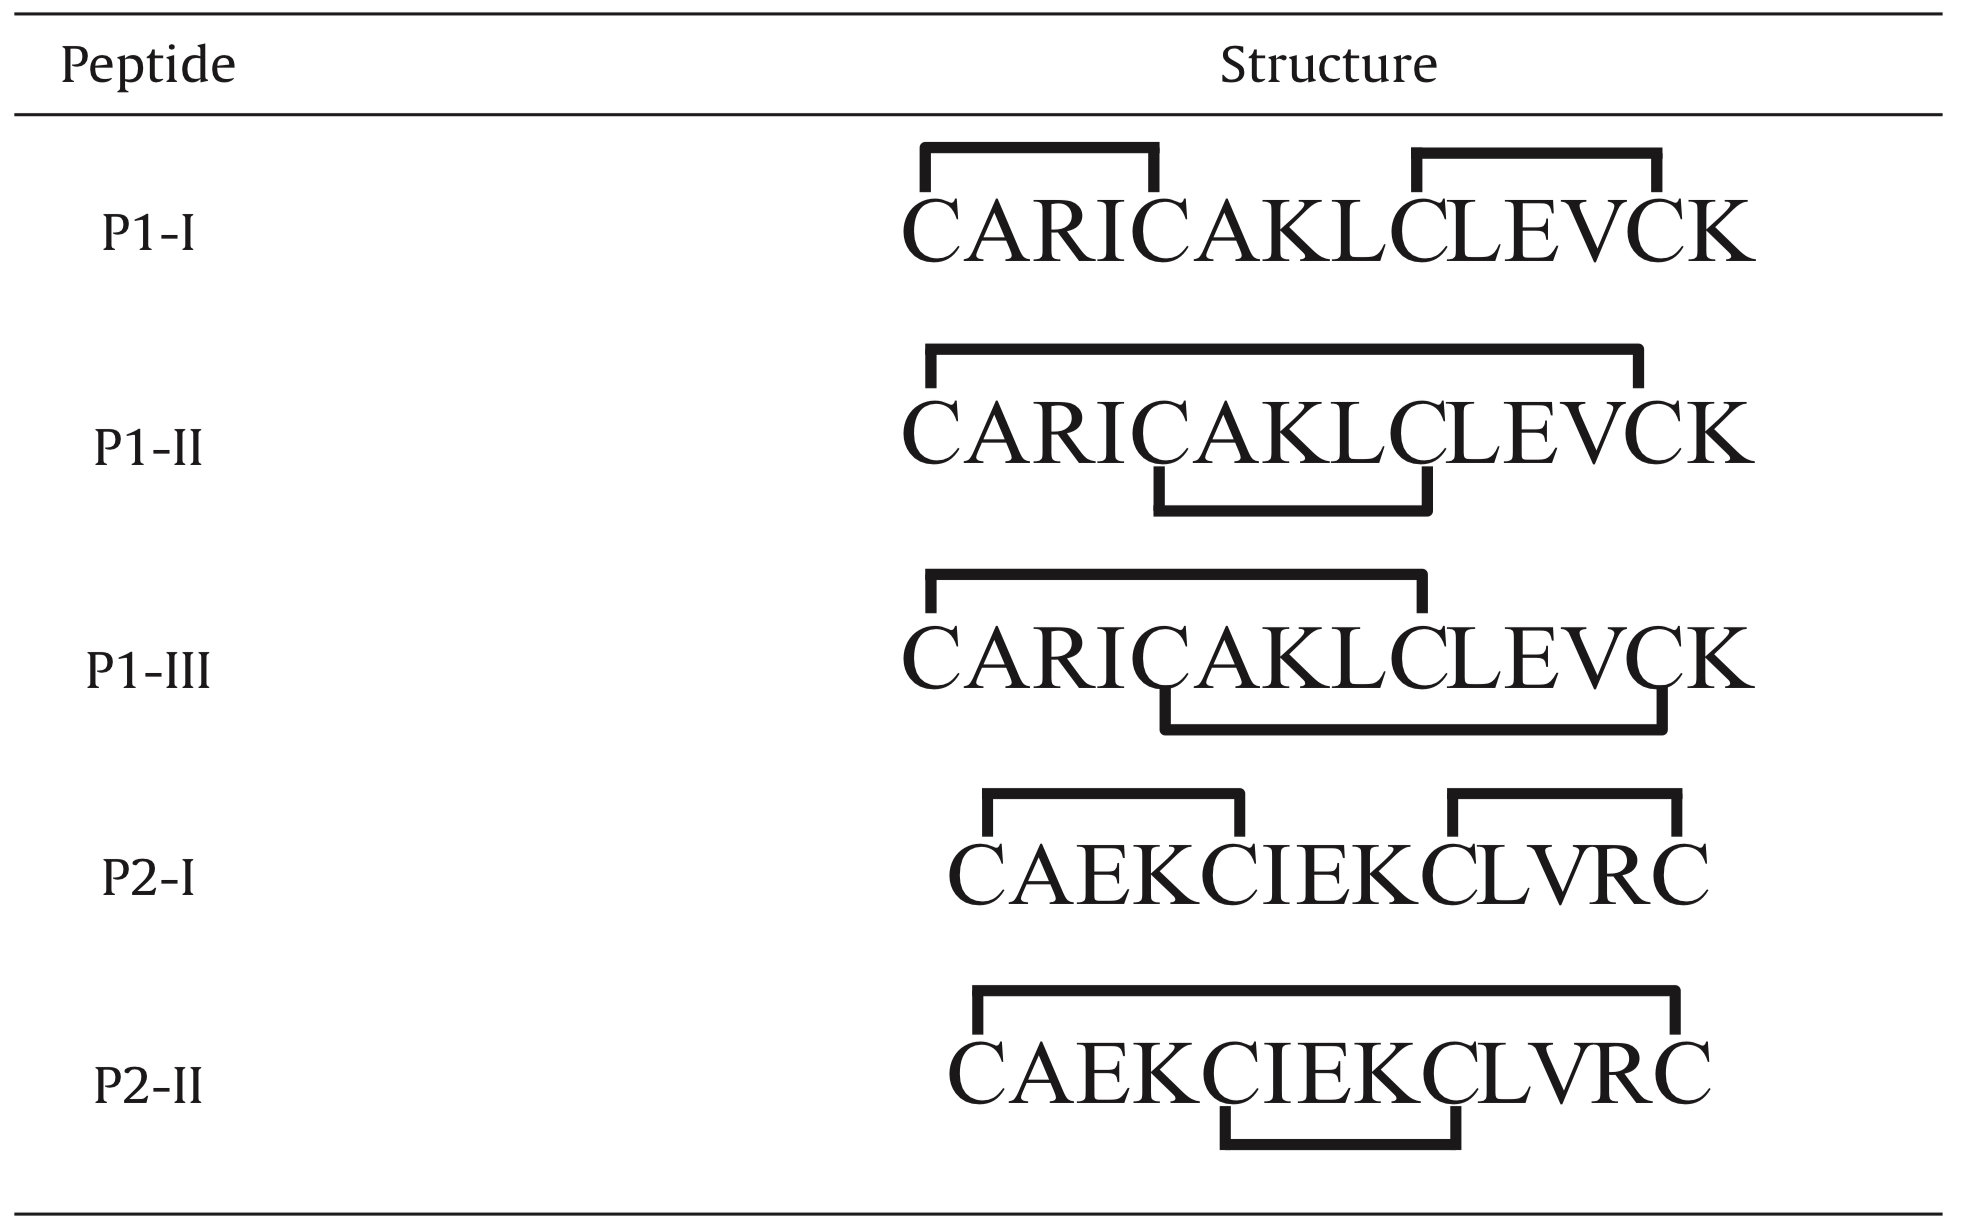
\includegraphics[width=.5\linewidth]{img/intrapeptide-bond.jpeg}
  \caption{An example of different possible configurations of intra-peptide \glspl*{db}. These types of precursors would be hard to discern by the common \gls*{db} mapping methods that rely on \gls*{db} dissociation, because the information about which cysteines were connected is lost. Image by~\citet{durand2013tandem}.}\label{fig:intra-peptide-bonds}
\end{figure}

If we managed to identify the cross-linked fragments (category 4) in the measured data, we would gain a lot of important evidence about the presence of certain \glspl*{db} in the protein. However, due to the complexity of the potential fragments, the fragment identification process is very hard to automate completely. The next section details some current approaches to fragment assignment and \gls*{db} mapping.

\section{Interpretation of fragmentation spectra of cross-linked peptides}\label{sec:analysis}

This section concerns itself with the existing methods that aim to determine the position of \glspl*{db} in a protein using \gls*{msms} data. After a short review of the manual and computation approaches to this problem, we formulate the task that this thesis is trying to solve in more precise terms, and finally perform a simple complexity analysis of the problem.

As noted by \citet{lakbub2018recent}, there are two main types of \gls*{db} characterization.

\begin{itemize}
  \item Profile comparison methods make use of two samples: one reduced with the \glspl*{db} removed, and one that is not reduced and the \glspl*{db} of which are still intact. Differential analysis is then deployed on a chromatogram profile of these two samples to determine which peptides are in the non-reduced, but are not in the reduced one. Those peptides are suspect of containing \glspl*{db} and are further analysed in \gls*{msms}\@.
  \item Intact analysis methods only use data from the non-reduced sample. Thus, they are simpler from the sample preparation standpoint, but have less information at their disposal than the profile comparison methods.
\end{itemize}

In each of the both categories, the protocols further differ in the choice of sample separation, ionization, and fragmentation methods, the choice of mass analyser, and whether the bulk of the analysis is performed manually or automatically~\cite{lakbub2018recent}. An example of a method that is partially manual now follows.

\citet{wu2009mass} propose an intact analysis method based on \gls*{lc}-\gls*{msms} with \gls*{etd}\@. The prepared peptides are measured on \gls*{ms}\textsuperscript{1}, and fragmented by \gls*{etd}\@. As described earlier, if the precursor ion contains \glspl*{db}, they are dissociated in \gls*{etd}, resulting in fragmentation spectra with two prominent peaks. The two peaks represent the two peptides that were connected by a \gls*{db} to become the original precursor ion. Fragments from these two peaks are put into an \gls*{ms}\textsuperscript{3} step that employs \gls*{cid} fragmentation to acquire their sequence information. This sidesteps the problem of not having data from the non-bound peptides in the intact methods. Software for fragment mass searching and matching is used, but because it is not made with \gls*{db} research in mind, the method requires frequent manual interventions.

It is likely that using specialized software for \gls*{db} mapping would be preferable in this scenario. We reviewed some current computational methods in the next section.

\subsection{Current computational approaches}

Dedicated \gls*{db} characterization software usually only needs data from non-reduced samples. Nonetheless, there are some commercial options that offer the possibility to add data from reduced samples, too, such as PepFinder and BioPharma Finder, as noted by \citet{lakbub2018recent}. The same authors offer a comprehensive list of past and current manual and computational \gls*{db} characterization methods.

SimXL is tool for general peptide cross-linking analysis~\cite{lima2015sim}, including \glspl*{db}~\cite{cui2019comprehensive}. SimXL has three main differentiating factors. First is the user-friendly UI that allows the researchers to view not only the interpreted results, but also the annotated data based on which they were computed. Second is its search space reduction heuristic based on the presence of a reporter ion~\cite{iglesias2010identification}, a peak that is specific to the fragmentation spectra of a cross-linked precursor. Finally, SimXL employs a further search space-reduction heuristic based on dead-end modifications, but we believe it is probably inapplicable in the context of \gls*{db} characterization.

A popular method by \citet{liu2014facilitating} includes a recommended research protocol, starting with protein digestion. Samples are digested with pepsin to avoid \gls*{db} scrambling, fragmented with \gls*{etd} followed by \gls*{hcd}, or (EThcD) for short, and finally analysed with SlinkS, a dedicated \gls*{db} matching algorithm. As mentioned previously, it is possible to extract information about the peptides constituting the precursor ion from the \gls*{etd} fragmentation spectra. The \gls*{hcd} step is employed in order to gain sequence information about these peptides, similarly to how \gls*{ms}\textsuperscript{3} has been used in~\cite{wu2009mass}.

Ultimately, thanks to EThcD, two peaks corresponding to the precursor peptide pair are identified in each fragmentation spectrum. Additionally, the whole precursor match is scored by scoring the fragments, now that it is known from which precursor they (allegedly) originated. The main shortcoming of this method is the fact that it only works with dipeptide precursors connected by a single \gls*{db}; it also ignores fragments with neutral loss and internal ion fragments. That makes it impossible to identify some of the more complicated \gls*{db} configurations, such as the ones in \Cref{fig:intra-peptide-bonds}.

In fact, all the aforementioned methods should be able to match simple inter-peptide \glspl*{db}, but they reportedly struggle with more complex \gls*{db} configurations~\cite{lakbub2018recent}; for some examples of complicated \gls*{db} configurations, see \Cref{fig:bond-types}.

A wide array of approaches to \glspl*{db} is offered, leading to a yet wider array of recommended sample preparation and fragmentation protocols. We conclude that computational \gls*{db} characterization is a hard problem to solve, a notion we formalize in the next section.

\begin{figure}
  \centering
  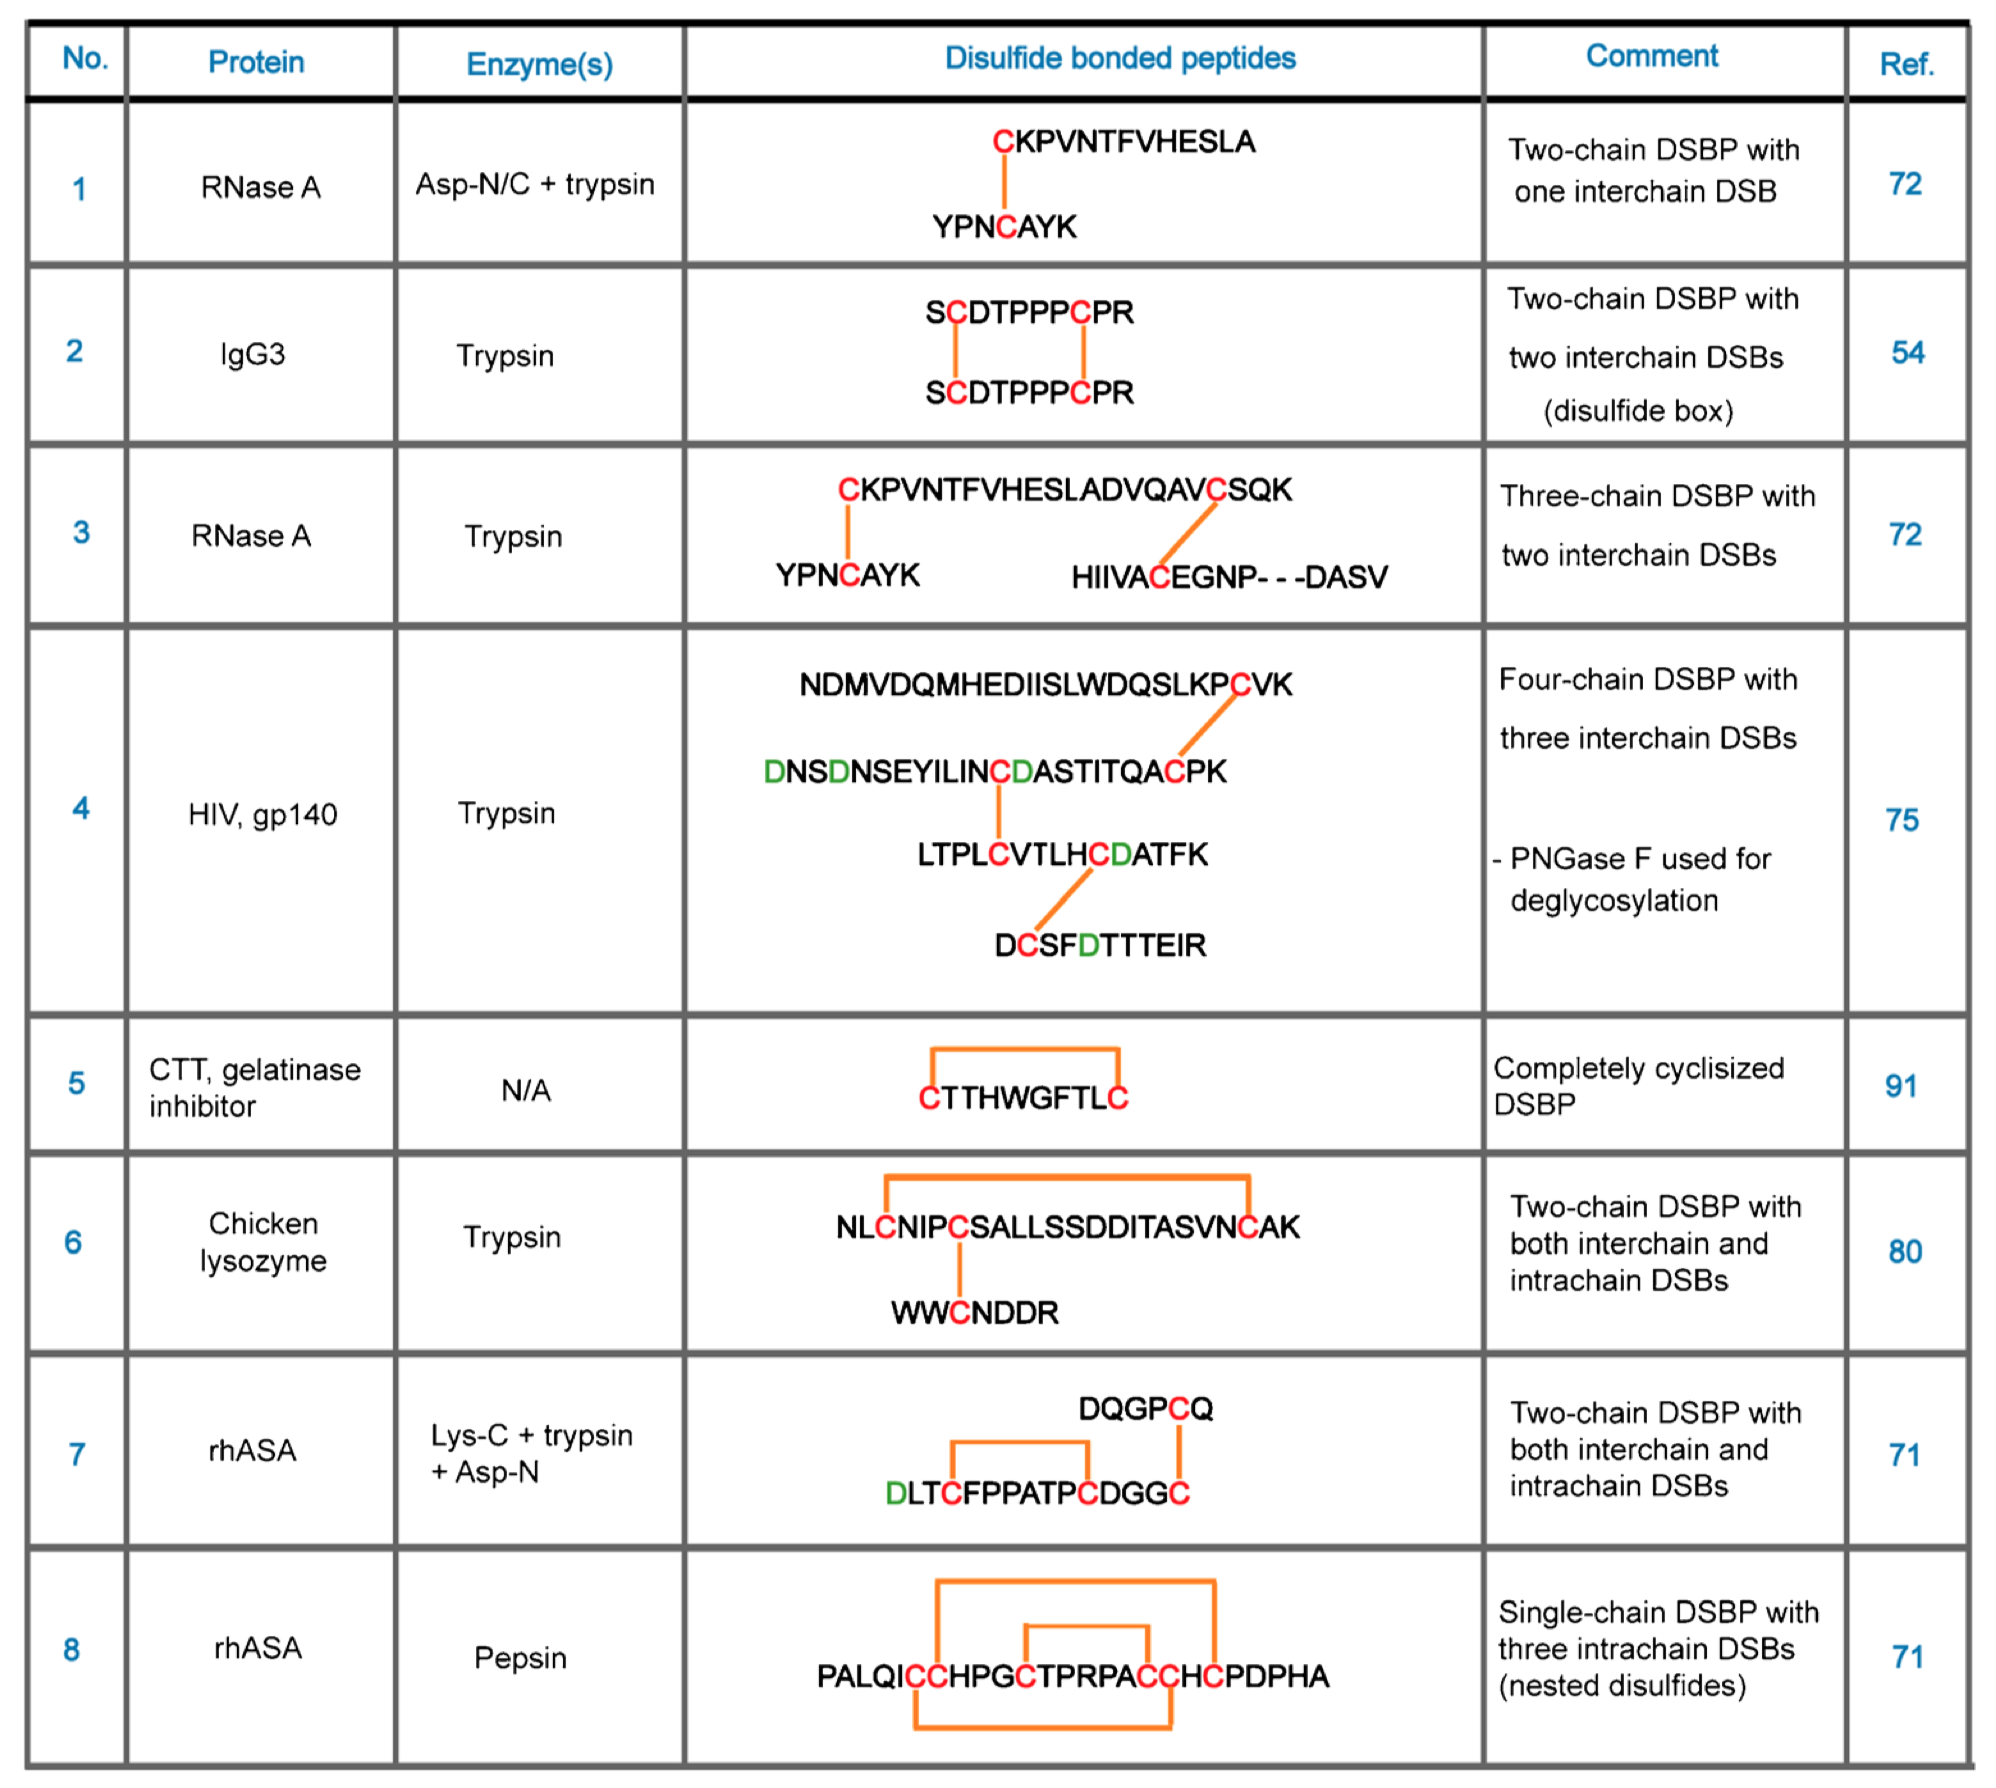
\includegraphics[width=1\linewidth]{img/bond-types.png}
  \caption{Illustrative examples of different ways peptides can be connected by disulphide bonds, ranging from relatively simple examples (1, 3, 5) to complex multi-peptide or multi-bond configurations (4, 8). The more complicated configurations proved to be hard to characterize computationally. Image by~\citet{lakbub2018recent}. (DSB = disulphide bond, gp140 = glycoprotein 140, rhASA = recombinant human arylsulfatase A)}\label{fig:bond-types}
\end{figure}


\subsection{Computational complexity of cross-linked fragment identification}

Indisputably, the problem of determining the characteristics of \gls*{db} linkages in proteins is hard. From biochemical point of view, already sample preparation poses a challenge; there is a need to minimize \gls*{db} scrambling, but at the same time have the protease be as specific as possible to simplify the subsequent analysis.

Another unresolved problem is the choice of dissociation method. \gls*{etd} spectra offer the information about the constituent peptides, which is useful when assigning precursor peptides. On the other hand, \gls*{cid}-based approaches have access to richer but more complicated fragmentation spectra, including interlinked fragments and internal ions with intact \glspl*{db}; these are useful for precise pinpointing of the \gls*{db} location.

To continue this discussion further, we need to be specific about the precise task we are attempting to solve. The ultimate goal is to determine where all \glspl*{db} in a protein are located, even if they are in complex configurations. In this thesis, we try to reach this goal by identifying a wide array of fragments in the measured fragmentation spectra, and aggregating the evidence they provide about positions of the individual \glspl*{db}. So, to solve the original \gls*{db} mapping problem, we need to be able to identify even complex fragments in \gls*{msms} data.

\subsubsection{A formalized perspective of the task}

We have a known precursor with defined \gls*{db} positions, that we will call a \emph{variant}, and a measured fragmentation spectrum. Our task is to say how well the variant matches the spectrum, by trying to assign in-silico generated fragments of the variant to the different measured peaks. Mathematically, we can represent the variant by a \emph{variant graph}.

\begin{defn}
  A \emph{variant graph} of a variant \(R\) comprising \(n\) residues is a graph \(G_R = (V, E)\) with weighted nodes, where \(V  = 1\ldots n\) and \((i, j) \in E\) if and only if there is a peptide or a \gls*{db} connecting  the \(i\)-th and \(j\)-th residue in \(R\). The weight \(w_i\) of the vertex \(i\) is the mass of the corresponding \(i\)-th residue in the precursor.
\end{defn}

The bonds in \(R\), and thus the edges in \(G_R\), are constrained in terms of connectivity --- there can be at most one \gls*{db} connected to a given residue, and at most two peptide bonds. However, \(G_R\) can still in theory be a relatively complex non-planar graph, as illustrated in \Cref{fig:nonplanar}.

\begin{figure}
  \centering
  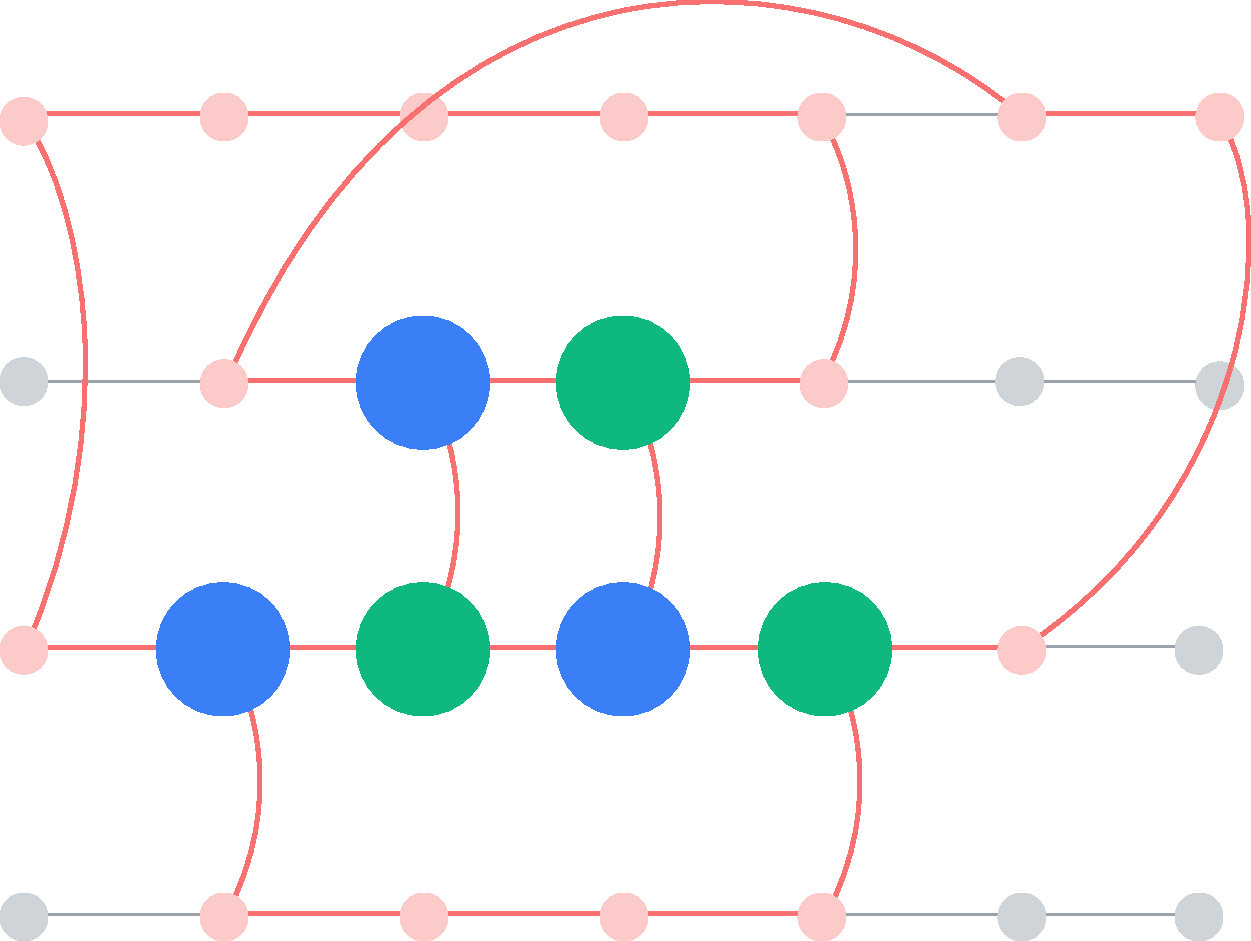
\includegraphics[width=0.5\linewidth]{img/nonplanar.pdf}
  \caption{An example of a valid precursor graph that is not planar due to the presence of a \(K_{3, 3}\) subdivision~\cite{kuratowski1930probleme} (highlighted). Vertices represent amino acid residues, horizontal lines represent peptide bonds, and vertical curved lines represent \glspl*{db}. The precursor could be made out of four different interlinked peptides, but it is also possible for it to be a single peptide with many intra-peptide \glspl*{db}.}\label{fig:nonplanar}
\end{figure}

\begin{defn}\label{defn:fragment}
  Given a fragment \(A\) of the variant \(R\), we will denote the connected subgraph representing the fragment in \(G_R\) as \(F_A\), and call it the \emph{fragment subgraph}. Every connected subgraph in \(G_R\) represents a fragment of \(R\).
\end{defn}

\begin{lemma}\label{lemma:mass}
  The number of cleavages that were required to create the fragment \(A\) is equal to the number of edges that have at least one vertex in \(F_A\), but are not themselves in its set of edges. The mass of \(A\) can be computed by summing up the weights of its vertices \(F_A\).
\end{lemma}

The task of matching the whole variant to a spectrum can be split into multiple subtasks of trying to find a fragment of the variant that matches a mass of a specific peak. By using \Cref{defn:fragment} and \Cref{lemma:mass} we can reformulate the subtask as searching for a connected subgraph in \(G_R\) in which the sum of vertex weights is equal to the mass of the peak we are trying to match. This problem is usually called the exact weight subgraph problem~\cite{abboud2013exact}, or, in our case, an exact weight \emph{connected} subgraph problem.

A well-studied closely related problem called the maximum weight connected k-subgraph problem was shown to be NP-hard on general graphs, and even on planar and bipartite graphs with integer weights~\cite{hochbaum1994node}.\footnote{The same authors propose a polynomial-time \(O(k^2n)\) dynamic programming algorithm for a restricted version of the problem searching for subgraphs in trees.} The exact weight connected subgraph problem has not been studied quite as thoroughly, but we believe it is safe to assume that its complexity will not be much lower. In other words, in the context of our not-necessarily-planar precursor graphs, the problem is likely NP-hard.

Furthermore, this was only a simplified look on the fragment matching problem. In reality, we are not looking for an exact match, but we have a tolerance range whose size is not absolute, but is defined relative to the mass of the generated fragment (in ppm). We also have to take into account the possible modifications of amino acid residues, the possible occurrences of a neutral loss, and the asymmetrical nature of \gls*{db} cleavage under \gls*{cid}, adding additional complexity to an already complex problem.

Nevertheless, in the next chapter we describe a general algorithm that attempts to solve the fragment matching problem, and use the results to identify \glspl*{db} in the original protein. We apply an upper bound on the number of cleavages of matched fragments, which limits the search space considerably. We also employ strict limits regarding the matching error, which enables us to search the space in a branch-and-bound fashion.